\section{Examples}
\paragraph{} The commands listed in the previous pages of this document are simple strings that can be sent to the Qube over its Serial Port, hence it is possible to establish the connection, send and receive commands, queries and replies with a variety of different programming languages and software.
\newline
Here we provide a couple simple example to show how to establish the communication with a QubeCL or QubeDL using different methods. In both cases, some of the previously described commands are used.


% ---------------    LabVIEW    ---------------

\subsection{LabVIEW}
\paragraph{} To control a Qube by the mean of a LabVIEW based control software, it is sufficient to properly configure a Serial COM port using the basic tools already provided by National Instrument.
\newline ppqSense made available a simple VI (Qube\textunderscore Serial\textunderscore Interface.vi) that can be integrated into a LabVIEW program in order to send and receive textual strings to a QubeCL with the proper format which can be downloaded from the website of requested to customer assistance (qube.support@ppqsense.odoo.com).

\begin{figure}[h]
    \centering
    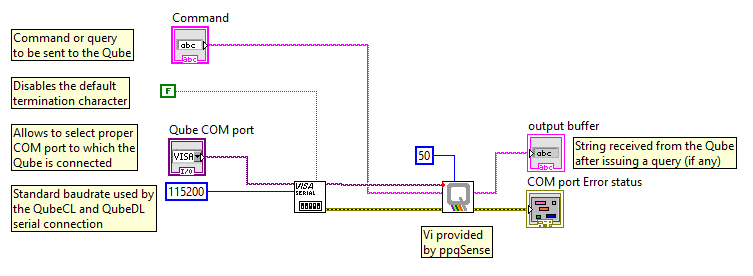
\includegraphics[width=15cm]{images/LabVIEW_VI_example.png}
    \caption{A simple LabVIEW program using the Qube\textunderscore Serial\textunderscore Interface.vi to communicate with a Qube}
    \label{LabVIEW_VI_example}
\end{figure}

\paragraph{} The Qube\textunderscore Serial\textunderscore Interface.vi needs a few inputs:
\begin{itemize}
    \item \textbf{Serial Port:} The serial port to which the Qube is connected, properly set up to work at 115200 baud without any termination character.
    \item \textbf{VISA Error:} The error for the VISA COM port made available by LabVIEW
    \item \textbf{Command:} A string containing the command with the \textbf{[identifier]:[value]} format to be sent to the Qube
    \item \textbf{Milliseconds to wait:} A constant defining how much time (in milliseconds) it is necessary to wait before accessing the Serial Buffer to read the reply received from the Qube (if any).
\end{itemize}

\paragraph{} The Qube\textunderscore Serial\textunderscore Interface.vi add the necessary terminating character in order for the command to be correctly executed by the Qube and gives back two outputs that can be used inside the program:

\begin{itemize}
    \item \textbf{Output buffer:} A string containing the reply from the Qube. It is empty for write commands or if the query gave no reply.
    \item \textbf{COM port Error status:} A VISA COM port error variable useful to check if anything went wrong during the communication with the Qube.
\end{itemize}

\begin{figure}[h]
    \centering
    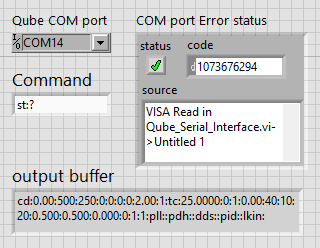
\includegraphics[width=7.5cm]{images/LabVIEW_CP_example.png}
    \caption{The panel screen of the same LabVIEW program used to send an \textbf{st:?} query to a Qube, showing the reply it sent back}
    \label{LabVIEW_CP_example}
\end{figure}


% ---------------    Python    ---------------

\subsection{Python}
\paragraph{} Python gives all the necessary tools to seamlessly connect to a Qube, sending commands and receiving replies to issued queries. As for the previous example, after a proper set up of the Serial connection, the communications is easy to implement.
\newline The example below shows a very simple function (\textit{write\textunderscore read\textunderscore from\textunderscore Qube}); it takes the command, with the \textbf{[identifier]:[value]} format, adds the necessary terminating character to it and send it to the Qube over a predefined Serial Port.
\newline The example also contains a simple script that uses the \textit{write\textunderscore read\textunderscore from\textunderscore Qube} function to perform a couple operations on the Qube.
\newline

\begin{lstlisting}[language=Python]
    import serial
    import time
    
    Qube_COM_num = "COM18"  #replace with the actual COM on your PC
    Qube_standard_Baudrate = 115200       #do not change!
    
    # initiate the serial connection
    Qube_Serial = serial.Serial(port = Qube_COM_num, baudrate = Qube_standard_Baudrate, timeout=0.6)
    
    
    
    # Basic fucntion to send commands to the Qube and receive reply to queries, if any
    def write_read_from_Qube(command):
        Qube_Serial.write(bytes(command + '\n', 'utf-8')) # adds the proper terminating character
        time.sleep(0.05)        # wait for 50 ms
        reply = Qube_Serial.readline().decode('utf8')
        return reply
    
    ########################################################################
    # Here a small demonstrative script to assess if a Qube is connected and working
    
    print("Testing the Serial Connection to the Qube")
    print("The Qube is connected to the Serial Port " + Qube_COM_num)
    print("The connection Baudrate is " + str(Qube_standard_Baudrate) + "\n")
    
    print("Issuing the command    id:?")
    Serial_number = write_read_from_Qube("id:?")
    print("The Serial Number of the Qube is: " + Serial_number)
    
    print("Checking the current status of the Qube by issuing the command   st:?\n")
    Qube_status = write_read_from_Qube("st:?")
    print("The Status of the Qube is: " + Qube_status)
    
    print("Setting the output current at 157 mA\n")
    write_read_from_Qube("iset:157")
    
    
    print("Checking if the setpoint for the output current has been received by issuing the command   st:?\n")
    Qube_status = write_read_from_Qube("st:?")
    print("The Status of the Qube is: " + Qube_status)
\end{lstlisting}

\newpage Once the proper COM port to use has been set, in this case COM18, it is possible to run the script and obtain a few information from the Qube, as shown below:

\begin{lstlisting}
    Testing the Serial Connection to the Qube
    The Qube is connected to the Serial Port COM18
    The connection Baudrate is 115200
    
    Issuing the command    id:?
    The Serial Number of the Qube is: QubeCL-185
    
    
    Checking the current status of the Qube by issuing the command   st:?
    
    The Status of the Qube is: 
        cd:810.03:900:2000:0:0:0:0:2.00:1:tc:5.0000:0:1:3.00:100:25:-10:
            0.500:0.221:0.000:1:1:1:pll::pdh::dds::pid::lkin:
    
    
    Setting the output current at 157 mA
    
    Checking if the setpoint for the output current has been received by issuing the command   st:?
    
    The Status of the Qube is:                      
        cd:157.00:900:2000:0:0:0:0:2.00:1:tc:5.0000:0:1:3.00:100:25:-10:0.500:
            0.221:0.000:1:1:1:pll::pdh::dds::pid::lkin:    
\end{lstlisting}